\documentclass{article}
\usepackage[utf8]{inputenc}
\usepackage{minted}
\usepackage{graphicx}
\usepackage{hyperref}
\usepackage[dvipsnames]{xcolor}
\usepackage{comment}

\title{lopy loramac gateway}
\author{cmonaton }
\date{August 2019}

\begin{document}

\maketitle

\section{Introduction}
But : Utiliser 3 lopy 4 pour envoyer des messages en point à point. 2 lopys communiquent avec 1 lopy gateway.

Carte : pycom lopy 4 avec expansion board V3.0



\begin{figure}[H]
  \centering
  \begin{minipage}[b]{0.4\textwidth}
    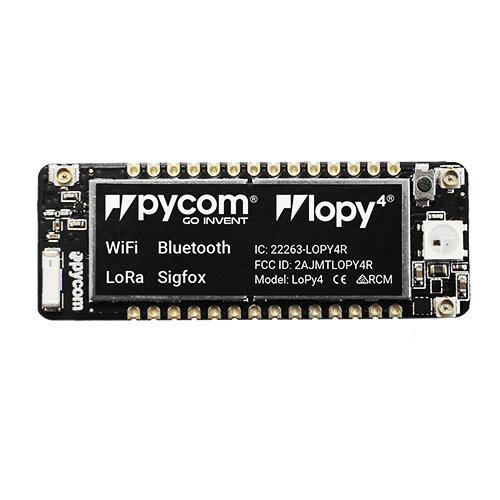
\includegraphics[keepaspectratio=true,scale=1.7]{pycom_lopy4.jpeg}
        \caption{pycom lopy 4}
  \end{minipage}
  \hfill
  \begin{minipage}[b]{0.4\textwidth}
   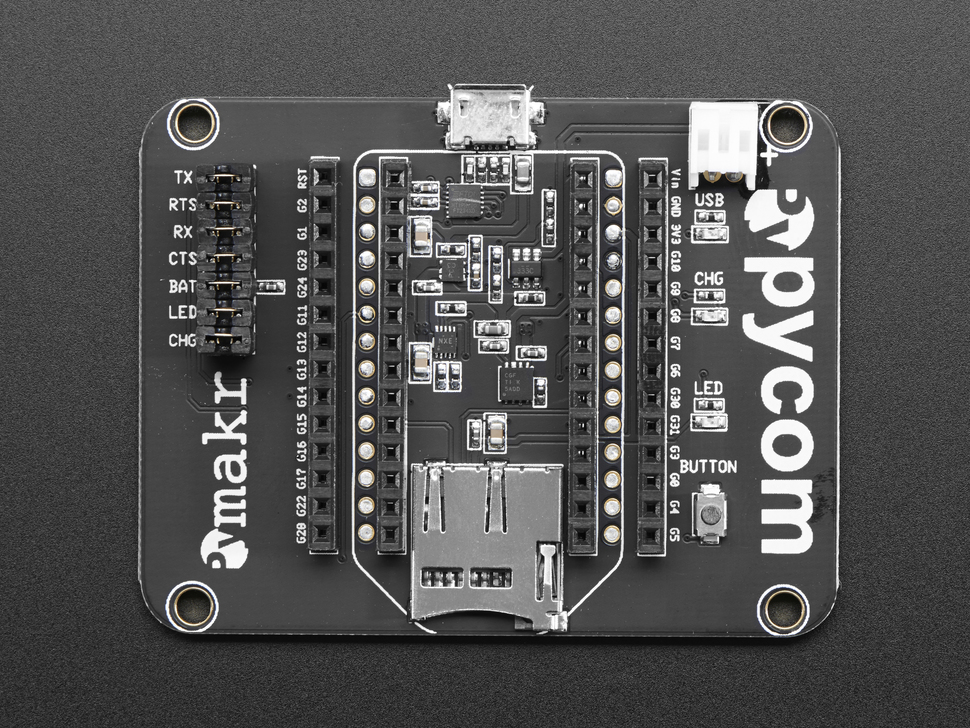
\includegraphics[keepaspectratio=true,scale=0.5]{pycom_expansion_board.jpeg}
    \caption{expansion board v3.0}
  \end{minipage}
\end{figure}

    \begin{figure}[H]
\begin{center}
\advance\leftskip-3cm
\advance\rightskip-3cm
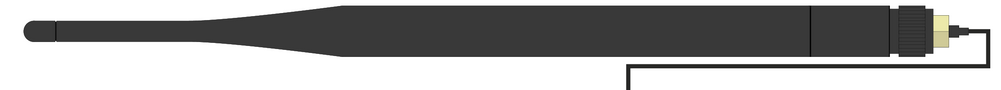
\includegraphics[keepaspectratio=true,scale=0.2]{lora_antenna.png}
\caption{antenne LoRa}
\label{visina8}
\end{center}\end{figure}



\section{Matériel}
\textcolor{red}{Branchez l'antenne LoRa avant d'alimenter la carte sinon la carte grille}

\section{Code}

Le code pour les 2 lopys et la gateway se trouve à : \url{https://github.com/GitClementtest/loramac_nanogateway}\\
Informations complémentaires : \url{https://docs.pycom.io/tutorials/lora/lorawan-nano-gateway/} 

\section{Télécharger le code sur les cartes}
\subsection{Installer ATOM et pymakr}

Télécharger la version 1.39.0 sur \url{https://github.com/atom/atom/releases/tag/v1.39.0}
Téléchargez le .deb. \\
\begin{comment}
\begin{minted}{bash}
wget -qO - https://packagecloud.io/AtomEditor/atom/gpgkey | sudo apt-key add -
sudo sh -c 'echo "deb [arch=amd64] https://packagecloud.io/AtomEditor/atom/any/ any main" 
> /etc/apt/sources.list.d/atom.list'
sudo apt-get update
sudo apt-get install atom



\end{minted}
atom pour lancer l'éditeur
\end{comment}
informations complémentaires à : \url{https://flight-manual.atom.io/getting-started/sections/installing-atom/#platform-linux}

\subsubsection{installer pymakr}


Depuis atom selon l'image installer pymakr


    \begin{figure}[H]
\begin{center}
\advance\leftskip-3cm
\advance\rightskip-3cm
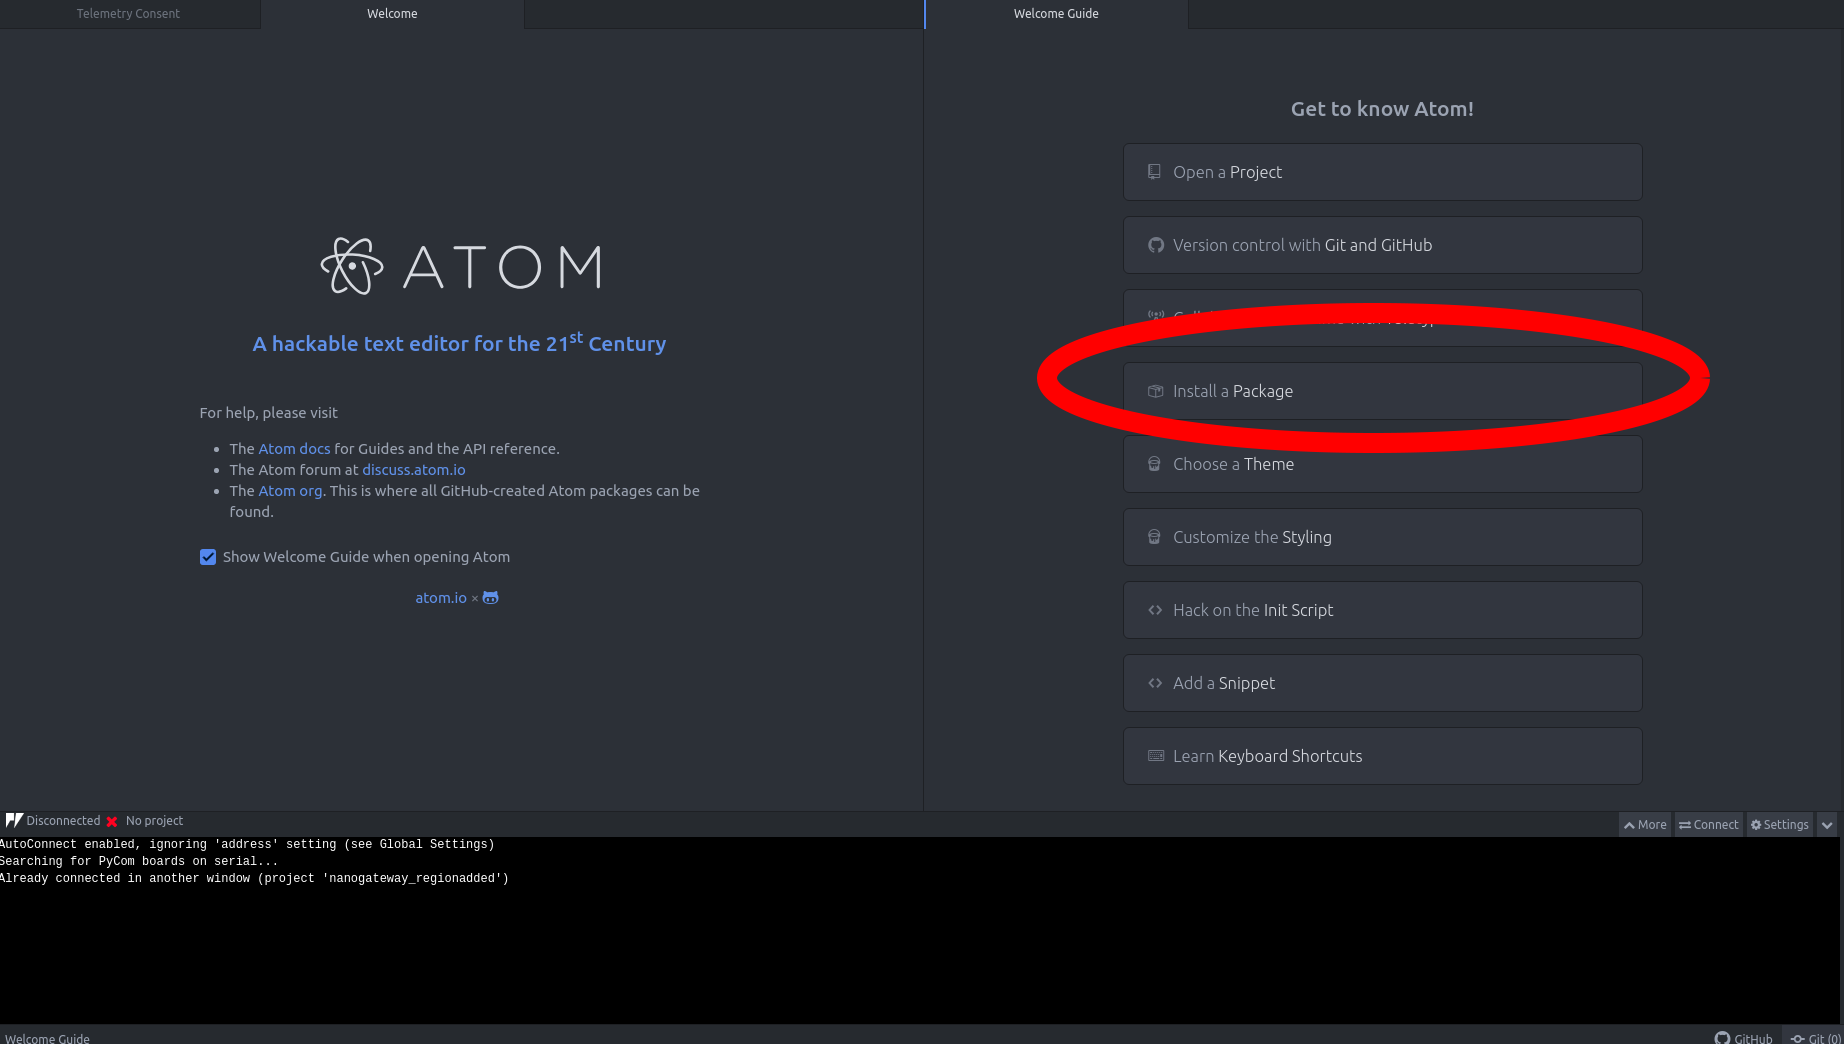
\includegraphics[keepaspectratio=true,scale=0.2]{atom_installpymakr.png}
\label{visina8}
\end{center}\end{figure}

Si il est impossible d'installer pymakr, installez une version antérieure à : \url{https://github.com/atom/atom/releases}\\
Désinstallez l'ancienne version :
\begin{minted}{bash}

sudo apt-get remove atom




\end{minted}

Pour ubuntu téléchargez le fichier .deb

Une alternative est aussi \textbf{Visual Studio Code}. \\

Informations complémentaires à  : \url{https://docs.pycom.io/pymakr/installation/atom/}

\subsection{Déverouiller les ports USB}
\subsubsection{Solution temporaire} 


\begin{minted}{bash}
sudo chmod 666 /dev/ttyACM0
\end{minted}
Il faut entrer cette commande souvent. \\
\subsubsection{Solution permanente}\\

Créer un fichier dans son home

\begin{minted}{bash}
50-myusb.rules
\end{minted} 

l'éditer : 

\begin{minted}{bash}
KERNEL=="ttyACM[0-9]*",MODE="0666"
\end{minted}

Puis copier ce fichier dans /etc/udev/rules.d/ et redémarrer votre PC.

\begin{minted}{bash}
 sudo cp 50-myusb.rules /etc/udev/rules.d
\end{minted}
C'est suffisant pour ne plus avoir à réouvrir les ports manuellement. Cependant, n'importe quel dispositif usb connecté au PC a maintenant le droit d'écriture sur le PC. \\

Pour plus de sécurité ajouter ces lignes dans ce fichier :

\begin{minted}{bash}
ACTION=="add", KERNEL=="ttyACM[0-9]*", ATTRS{idVendor}=="xxxx", 
ATTRS{idProduct}=="yyyy", MODE="0666"
\end{minted}
 
 Pour déterminer idVendor et idProduct des cartes tapez lsusb avant et après avoir connecté la carte. \\

 Dans mon cas :
 
 \begin{figure}[H]
\begin{center}
\advance\leftskip-3cm
\advance\rightskip-3cm
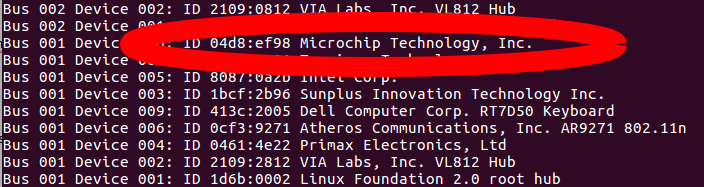
\includegraphics[keepaspectratio=true,scale=0.5]{lsusb.png}
\label{visina8}
\end{center}\end{figure}

idProduct = ef98\\
idVendor= 04d8\\







\section{Communication entre la gateway et les lopys}

Connectez-vous avec minicom ou putty aux lopys ports ttyACM0,1,2 avec le réglage 115200 8N1, voilà ce qu'on observe : \\

 \begin{figure}[H]
\begin{center}
\advance\leftskip-3cm
\advance\rightskip-3cm
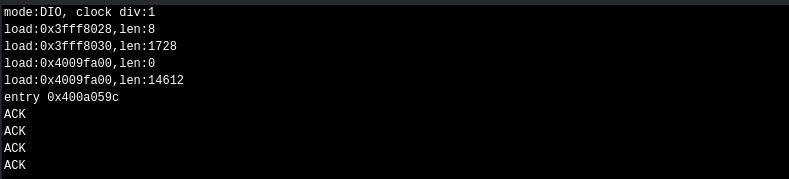
\includegraphics[keepaspectratio=true,scale=0.5]{gatewayloramac_ack.png}
\caption{Lopys A et B}
\label{visina8}
\end{center}\end{figure}



 \begin{figure}[H]
\begin{center}
\advance\leftskip-3cm
\advance\rightskip-3cm
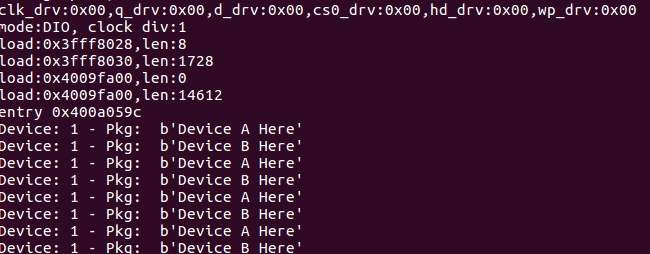
\includegraphics[keepaspectratio=true,scale=0.5]{gateway_loramac_deviceABhere.png}
\caption{nanogateway}
\label{visina8}
\end{center}\end{figure}

Pour utiliser Minicom : \\
Pour quitter minicom :
\begin{minted}{bash}
ctrl+a puis q

\end{minted}
Pour configurer minicom : 
\begin{minted}{bash}
sudo minicom -s

\end{minted}

Configuration de la liaison série :

\begin{figure}[H]
\begin{center}
\advance\leftskip-3cm
\advance\rightskip-3cm
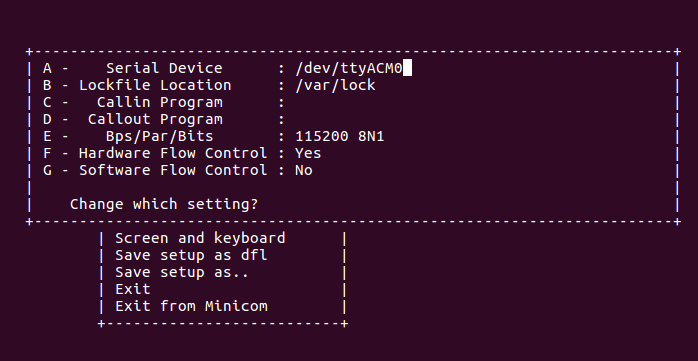
\includegraphics[keepaspectratio=true,scale=0.5]{loramacgateway_minicomconfig.png}
%\caption{nanogateway}
\label{visina8}
\end{center}\end{figure}


\end{document}
